%%%%%%%%%%%%%%%%%%%%%%%%%%%%%%%%%%%%%%%%%
% Stata Markdown: Creating Reproducible Reports
% Theme: CambridgeUS
%%%%%%%%%%%%%%%%%%%%%%%%%%%%%%%%%%%%%%%%%

\documentclass[dvipsnames,hyperref={pdfpagelabels=false}]{beamer}
\usepackage{ragged2e}
\renewcommand{\raggedright}{\leftskip=0pt \rightskip=0pt plus 0cm}
\usepackage{listings}
\usepackage{lmodern}
\usepackage{fontspec}
\usepackage{xeCJK}
\setCJKmainfont{Noto Sans CJK TC}
\setCJKsansfont{Noto Sans CJK TC}
\setCJKmonofont{Noto Sans Mono CJK TC}
\usepackage[english]{babel}
\usepackage{amsmath,amssymb,amsfonts,amsthm}
\hypersetup{colorlinks=true,urlcolor=blue,citecolor=blue,pdfborder={0 0 0}}
\usepackage{tikz}
\usetikzlibrary{arrows.meta,positioning,shapes.geometric}
\usepackage{booktabs}
\usepackage{xcolor}
\usepackage{colortbl}

\lstdefinelanguage{Stata}{
  morekeywords=[3]{regress,summarize,display,use,gen,replace,drop,capture,cd,markstat,whereis,ssc,install,global},
  morekeywords=[4]{if,foreach,forvalues,set},
  morecomment=[l]{//},
  morecomment=[s]{/*}{*/},
  morestring=[b]",
  sensitive=true,
}
\lstdefinestyle{stata-slide}{
  language=Stata,
  basicstyle=\footnotesize\ttfamily,
  keywordstyle=[3]{\color{NavyBlue}},
  keywordstyle=[4]{\color{NavyBlue}},
  stringstyle=\color{Maroon},
  commentstyle=\color{OliveGreen},
  breaklines=true,
  frame=single,
  numbers=none,
  showstringspaces=false,
  backgroundcolor=\color{gray!6},
}
\lstset{style=stata-slide}

% ---- Theme block ----
\usetheme{CambridgeUS}
\setbeamertemplate{footline}{%
  \hfill\usebeamercolor[fg]{page number in head/foot}%
  \usebeamerfont{page number in head/foot}%
  \insertframenumber\,/\,\inserttotalframenumber\hspace{1em}\vspace{2pt}%
}
\beamersetuncovermixins{\opaqueness<1>{25}}{\opaqueness<2->{15}}

\title[]{Stata Markdown \\ Creating Reproducible Reports}
\author{Prof.\ Tzu-Ting Yang \\ 楊子霆}
\institute{Institute of Economics, Academia Sinica \\ 中央研究院經濟研究所}
\date{\today}

\begin{document}

% ============================================================
% 1. Title frame
% ============================================================
\begin{frame}{}
  \titlepage
\end{frame}

% ============================================================
% Section divider: What Is Stata Markdown?
% ============================================================
\title[]{What Is Stata Markdown?}
\author{}\institute{}\date{}
\begin{frame}{}
  \titlepage
\end{frame}

% ============================================================
% 3. Frame: What Is Stata Markdown?
% ============================================================
\begin{frame}{What Is Stata Markdown?}
  \begin{itemize}
    \item A \texttt{.stmd} file mixes narrative text (Markdown) + Stata code blocks
    \item When compiled: Stata runs the code, captures output \& figures
    \item Pandoc converts the result into a polished \textbf{HTML} (or PDF) report
    \item Similar to R Markdown --- but for Stata
  \end{itemize}

  \vspace{0.8em}
  \begin{center}
    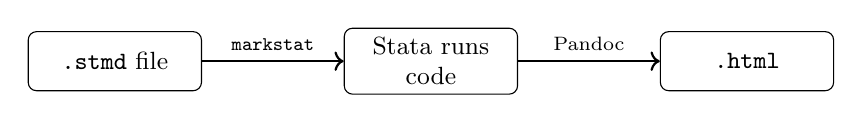
\begin{tikzpicture}[
        node distance=1.8cm,
        box/.style={rectangle, draw, rounded corners=3pt,
                    minimum width=2.2cm, minimum height=0.75cm,
                    align=center, font=\small},
        lbl/.style={font=\scriptsize, above}
      ]
      \node[box] (stmd) {\texttt{.stmd} file};
      \node[box, right=of stmd] (stata) {Stata runs\\code};
      \node[box, right=of stata] (html) {\texttt{.html}};

      \draw[->, thick] (stmd) -- node[lbl]{\texttt{markstat}} (stata);
      \draw[->, thick] (stata) -- node[lbl]{Pandoc} (html);
    \end{tikzpicture}
  \end{center}
\end{frame}

% ============================================================
% 4. Frame: Why Use Stata Markdown?
% ============================================================
\begin{frame}{Why Use Stata Markdown?}
  \begin{itemize}
    \item \textbf{One file, everything inside}: code + output + figures + explanation
          in a single self-contained \texttt{.html}
    \item \textbf{Fully reproducible}: re-running the \texttt{.stmd} always regenerates
          the same report
    \item \textbf{Easy to submit}: one \texttt{.html} captures your entire empirical
          workflow
  \end{itemize}

  \vspace{1em}
  \begin{center}
    \alert{Goal: produce one \texttt{.html} file recording all code and results}
  \end{center}
\end{frame}

% ============================================================
% Section divider: Course Templates on Dropbox
% ============================================================
\title[]{Course Templates on Dropbox}
\author{}\institute{}\date{}
\begin{frame}{}
  \titlepage
\end{frame}

% ============================================================
% 6. Frame: Course Templates on Dropbox
% ============================================================
\begin{frame}{Course Templates on Dropbox}
  \begin{center}
    \begin{tabular}{ll}
      \toprule
      \textbf{Folder} & \textbf{Contents} \\
      \midrule
      \texttt{do/} & Regular \texttt{.do} files --- reference for Stata code \\
      \texttt{do/Stata\_Markdown/} & Ready-to-compile \texttt{.stmd} templates --- \textbf{main reference} \\
      \bottomrule
    \end{tabular}
  \end{center}

  \vspace{1em}
  Open the \texttt{.stmd} template closest to your method and follow its structure.
\end{frame}

% ============================================================
% 7. Frame: Available .stmd Templates
% ============================================================
\begin{frame}{Available \texttt{.stmd} Templates}
  \begin{columns}[t]
    \column{0.48\textwidth}
    \begin{itemize}
      \item \texttt{regression.stmd}
      \item \texttt{DID.stmd}
      \item \texttt{Stag\_DID.stmd}
      \item \texttt{Syn\_DID.stmd}
      \item \texttt{fixed\_effects.stmd}
      \item \texttt{matching.stmd}
    \end{itemize}

    \column{0.48\textwidth}
    \begin{itemize}
      \item \texttt{RDD.stmd}
      \item \texttt{IV.stmd}
      \item \texttt{SSIV.stmd}
      \item \texttt{SCM.stmd}
      \item \texttt{ML.stmd}
    \end{itemize}
  \end{columns}

  \vspace{1em}
  \begin{center}
    \alert{Each template is a complete working example $\to$ compile it first,
    then adapt to your own data}
  \end{center}
\end{frame}

% ============================================================
% Section divider: One-Time Setup
% ============================================================
\title[]{One-Time Setup}
\author{}\institute{}\date{}
\begin{frame}{}
  \titlepage
\end{frame}

% ============================================================
% 9. Frame: What You Need to Install
% ============================================================
\begin{frame}{What You Need to Install}
  \begin{center}
    \begin{tabular}{lll}
      \toprule
      \textbf{Step} & \textbf{What} & \textbf{Where} \\
      \midrule
      1 & \texttt{markstat} Stata package & Inside Stata \\
      2 & \texttt{whereis} Stata package  & Inside Stata \\
      3 & Pandoc (external program)       & Your operating system \\
      4 & Register Pandoc with Stata      & Stata Command window (once) \\
      \bottomrule
    \end{tabular}
  \end{center}

  \vspace{1em}
  \textit{Steps 1--2 take 30 seconds. Steps 3--4 are the ones most often missed.}
\end{frame}

% ============================================================
% 10. Frame: Steps 1 & 2 --- Install Stata Packages [fragile]
% ============================================================
\begin{frame}[fragile]{Steps 1 \& 2 --- Install Stata Packages}
  Run once in the Stata Command window:
  \begin{lstlisting}
ssc install markstat, replace
ssc install whereis,  replace
  \end{lstlisting}

  \begin{itemize}
    \item \texttt{markstat}: reads \texttt{.stmd}, runs Stata code, calls Pandoc
    \item \texttt{whereis}: tells Stata where to find Pandoc
    \item \texttt{, replace} is safe to re-run
  \end{itemize}

  \vspace{0.5em}
  Verify: type \texttt{which markstat} --- if it prints a path, done \checkmark
\end{frame}

% ============================================================
% 11. Frame: Step 3 --- Install Pandoc
% ============================================================
\begin{frame}{Step 3 --- Install Pandoc}
  \begin{itemize}
    \item Pandoc is a \textbf{free, open-source} document converter
    \item It converts Stata output into formatted \textbf{HTML} or \textbf{PDF}
    \item Must be installed \textbf{outside Stata}, like any regular application
    \item Download: \url{https://pandoc.org/installing.html}
  \end{itemize}

  \vspace{1em}
  \alert{Important}: Installing Pandoc does NOT tell Stata where it is $\to$ that is Step 4
\end{frame}

% ============================================================
% 12. Frame: Step 3 --- Pandoc on Windows [fragile]
% ============================================================
\begin{frame}[fragile]{Step 3 --- Pandoc on Windows}
  \begin{enumerate}
    \item Go to \texttt{pandoc.org} $\to$ download the \texttt{.msi} installer $\to$ run it
    \item Open \textbf{Command Prompt} (search ``cmd'' in Start menu) and type:
  \end{enumerate}

  \begin{lstlisting}[language={},backgroundcolor=\color{gray!6}]
where pandoc
  \end{lstlisting}

  \begin{enumerate}
    \setcounter{enumi}{2}
    \item Copy the path printed (e.g.\
          \texttt{C:\textbackslash Users\textbackslash YourName\textbackslash AppData\textbackslash Local\textbackslash Pandoc\textbackslash pandoc.exe})
    \item You will need this exact path in Step 4
  \end{enumerate}
\end{frame}

% ============================================================
% 13. Frame: Step 3 --- Pandoc on macOS [fragile]
% ============================================================
\begin{frame}[fragile]{Step 3 --- Pandoc on macOS}
  \textbf{Option A} (Homebrew, recommended): open Terminal and run:
  \begin{lstlisting}[language={},backgroundcolor=\color{gray!6}]
brew install pandoc
which pandoc
  \end{lstlisting}
  Common result: \texttt{/usr/local/bin/pandoc} (Intel) or
  \texttt{/opt/homebrew/bin/pandoc} (Apple Silicon)

  \vspace{0.5em}
  \textbf{Option B}: download \texttt{.pkg} from \texttt{pandoc.org}

  \vspace{0.5em}
  Verify (any OS):
  \begin{lstlisting}[language={},backgroundcolor=\color{gray!6}]
pandoc --version
  \end{lstlisting}
  Should print \texttt{pandoc 3.x.x}
\end{frame}

% ============================================================
% 14. Frame: Step 4 --- Register Pandoc with Stata [fragile]
% ============================================================
\begin{frame}[fragile]{Step 4 --- Register Pandoc with Stata}
  \alert{\textbf{This is the step most students miss!}}

  \vspace{0.5em}
  Run ONCE in the Stata \textbf{Command window} (NOT inside a do-file):

  \smallskip
  Windows (adjust path to match yours):
  \begin{lstlisting}
whereis pandoc "C:\Users\YourName\AppData\Local\Pandoc\pandoc.exe"
  \end{lstlisting}

  macOS Intel:
  \begin{lstlisting}
whereis pandoc "/usr/local/bin/pandoc"
  \end{lstlisting}

  macOS Apple Silicon:
  \begin{lstlisting}
whereis pandoc "/opt/homebrew/bin/pandoc"
  \end{lstlisting}

  \vspace{0.3em}
  This registration is \textbf{permanent} --- you only need to do it once per machine.

  \vspace{0.3em}
  Verify: type \texttt{whereis pandoc} again (no path argument) --- should print
  your registered path \checkmark
\end{frame}

% ============================================================
% Section divider: Writing Your .stmd File
% ============================================================
\title[]{Writing Your \texttt{.stmd} File}
\author{}\institute{}\date{}
\begin{frame}{}
  \titlepage
\end{frame}

% ============================================================
% 16. Frame: Structure of a .stmd File [fragile]
% ============================================================
\begin{frame}[fragile]{Structure of a \texttt{.stmd} File}
  \begin{enumerate}
    \item \textbf{YAML header} (between \texttt{-{}-{}-} lines): title, author, date
    \item \textbf{Markdown text}: narrative explanation, section headings (\texttt{\#\#})
    \item \textbf{Stata code blocks}: fenced with \texttt{`{}``s} \ldots{} \texttt{`{}``}
  \end{enumerate}

  \vspace{0.5em}
  \begin{lstlisting}[language={},backgroundcolor=\color{gray!6}]
---
title: "My Report"
author: "Your Name"
---

## 1. Load Data

```s
use "$rawdata/mydata.dta", clear
summarize
```
  \end{lstlisting}
\end{frame}

% ============================================================
% 17. Frame: Types of Code Blocks
% ============================================================
\begin{frame}{Types of Code Blocks}
  \begin{center}
    \begin{tabular}{llll}
      \toprule
      \textbf{Syntax} & \textbf{Code shown} & \textbf{Output shown} & \textbf{Use for} \\
      \midrule
      \texttt{`{}``s}     & Yes & Yes & All analysis steps \\
      \texttt{`{}``s/q}   & No  & No  & Setup, path config, \texttt{ssc install} \\
      \texttt{`{}``} (plain) & Yes & Not run & Showing commands as reference only \\
      \bottomrule
    \end{tabular}
  \end{center}
\end{frame}

% ============================================================
% 18. Frame: Portable Path Setup [fragile]
% ============================================================
\begin{frame}[fragile]{Portable Path Setup}
  \textbf{Problem}: hard-coded paths break when shared with others.

  \textbf{Solution}: use \texttt{c(username)}.

  \begin{lstlisting}
```s/q
if "`c(username)'" == "alice" {
    global rawdata = "C:\Users\alice\Desktop\data"
}
if "`c(username)'" == "bob" {
    global rawdata = "/Users/bob/Documents/data"
}
```
  \end{lstlisting}

  \vspace{0.5em}
  Find your username: type
  \texttt{display \textasciigrave c(username)\textquotesingle}
  in the Stata Command window.
\end{frame}

% ============================================================
% Section divider: Compile to HTML
% ============================================================
\title[]{Compile to HTML}
\author{}\institute{}\date{}
\begin{frame}{}
  \titlepage
\end{frame}

% ============================================================
% 20. Frame: Compile --- Two Commands [fragile]
% ============================================================
\begin{frame}[fragile]{Compile --- Two Commands}
  \textbf{Step 1} --- change to the folder containing your \texttt{.stmd}:
  \begin{lstlisting}
cd "C:\Users\YourName\Desktop\MyProject"
  \end{lstlisting}

  \textbf{Step 2} --- compile:
  \begin{lstlisting}
markstat using myreport, bundle
  \end{lstlisting}

  \begin{itemize}
    \item Replace \texttt{myreport} with your filename (\textbf{no} \texttt{.stmd} extension)
    \item \texttt{bundle}: embeds all figures directly into the HTML $\to$ one portable file
    \item Output: \texttt{myreport.html} in the same folder
  \end{itemize}

  \vspace{0.5em}
  \begin{center}
    \alert{Open \texttt{myreport.html} in any browser --- done!}
  \end{center}
\end{frame}

% ============================================================
% 21. Frame: The bundle Option
% ============================================================
\begin{frame}{The \texttt{bundle} Option}
  \textbf{Without} \texttt{bundle}:
  \begin{itemize}
    \item HTML references external image files
    \item Images break when you move or submit the file
  \end{itemize}

  \vspace{0.5em}
  \textbf{With} \texttt{bundle}:
  \begin{itemize}
    \item All figures embedded directly as Base64 inside the HTML
    \item Single self-contained file --- nothing else needed
    \item \textbf{Always use \texttt{bundle} for homework submission}
  \end{itemize}
\end{frame}

% ============================================================
% Section divider: Troubleshooting
% ============================================================
\title[]{Troubleshooting}
\author{}\institute{}\date{}
\begin{frame}{}
  \titlepage
\end{frame}

% ============================================================
% 23. Frame: Common Errors
% ============================================================
\begin{frame}{Common Errors}
  \small
  \begin{center}
    \begin{tabular}{lll}
      \toprule
      \textbf{Error} & \textbf{Cause} & \textbf{Fix} \\
      \midrule
      \texttt{pandoc not found}        & Not registered      & \texttt{whereis pandoc "path"} \\
      \texttt{markstat unrecognized}   & Not installed       & \texttt{ssc install markstat} \\
      \texttt{whereis unrecognized}    & Not installed       & \texttt{ssc install whereis} \\
      file not found (compile)         & Wrong directory     & \texttt{cd} to folder with \texttt{.stmd} \\
      Images missing in HTML           & Missing \texttt{bundle} & \texttt{markstat using file, bundle} \\
      Variable already defined         & Code ran twice      & \texttt{capture drop varname} before \texttt{gen} \\
      \bottomrule
    \end{tabular}
  \end{center}
\end{frame}

% ============================================================
% Section divider: Summary
% ============================================================
\title[]{Summary}
\author{}\institute{}\date{}
\begin{frame}{}
  \titlepage
\end{frame}

% ============================================================
% 25. Frame: Setup Checklist
% ============================================================
\begin{frame}{Setup Checklist}
  \begin{enumerate}
    \item $\square$ \texttt{ssc install markstat, replace}
    \item $\square$ \texttt{ssc install whereis, replace}
    \item $\square$ Install Pandoc from \url{pandoc.org}
    \item $\square$ Find path: \texttt{where pandoc} (Windows) / \texttt{which pandoc} (macOS)
    \item $\square$ \textbf{Register}: \texttt{whereis pandoc "full/path"} \quad
          (Command window, once!)
    \item $\square$ Write \texttt{.stmd} file (YAML + Markdown + \texttt{`{}``s} blocks)
    \item $\square$ \texttt{cd "folder\textbackslash with\textbackslash your\textbackslash stmd"}
    \item $\square$ \texttt{markstat using yourfile, bundle}
    \item $\square$ Open \texttt{yourfile.html} in browser $\checkmark$
  \end{enumerate}
\end{frame}

\end{document}
